\chapter{DUNE Project Management}
\label{ch:detectors-pm}

\fixme{Is this really intended just for DUNE Project, or for other management structures 
within the Collaboration, too?  It needs to jive with vol 1 chap 4 in either case.  Eric and/or 
CKJ should revisit this  before anyone else reviews it, I think. (Anne)} 

\section{Overview}

As discussed in \volintro, the DUNE Project is part of the DUNE
Collaboration. The Project receives appropriate oversight from
stakeholders including the Collaboration and DOE. The Project is
responsible for the entire international project scope and will manage
this scope matching DOE requirements. The DUNE Project has its Project Office
headquartered at Fermilab.
The Project manages the design, construction, installation and
commissioning of the DUNE near and far detectors.

The entire DUNE Project (including international contributions)
will be subject to the DOE critical decision process incorporating a
CD-2 baseline cost and schedule approval and a CD-3 start of construction approval.

The Project will directly manage DOE project funds and any common
funds collected from U.S. and international stakeholders. The
DOE-funded portion will be managed in a manner that satisfies DOE
requirements and the international portion will be managed in a
similar manner tailored to each nation's requirements. It is expected
that Project funding obtained through other agencies will be managed
by groups set up by those agencies.

The Project is responsible for monitoring and reporting the status of
all contributions to the Project independent of their funding source,
at least to the level of subproject milestones.  Non-DOE partners will
report progress on their contributions to the Project Office as
defined in formal Memoranda of Understanding (MOU).

\section[Work Breakdown Structure (WBS)]{WBS}

The DUNE Project will manage all contributions to the design,
construction, installation and commissioning of the DUNE near and far
detectors through an international Work Breakdown Structure (WBS).
The WBS organizes the Project's tasks and deliverables into convenient
components and is used to organize the cost and schedule for the DUNE
project. The DUNE Project consists of two major subsystems: the Near Detector
(WBS 130.03), shown to WBS level 4 in Figure~\ref{fig:ND_WBS}, and the
Far Detector (WBS 130.05), shown to WBS level 3 in
Figure~\ref{fig:FD_WBS}.
\begin{cdrfigure}[Near detector WBS]{ND_WBS}{Near detector Work Breakdown Structure.}
\centering
\begin{center}
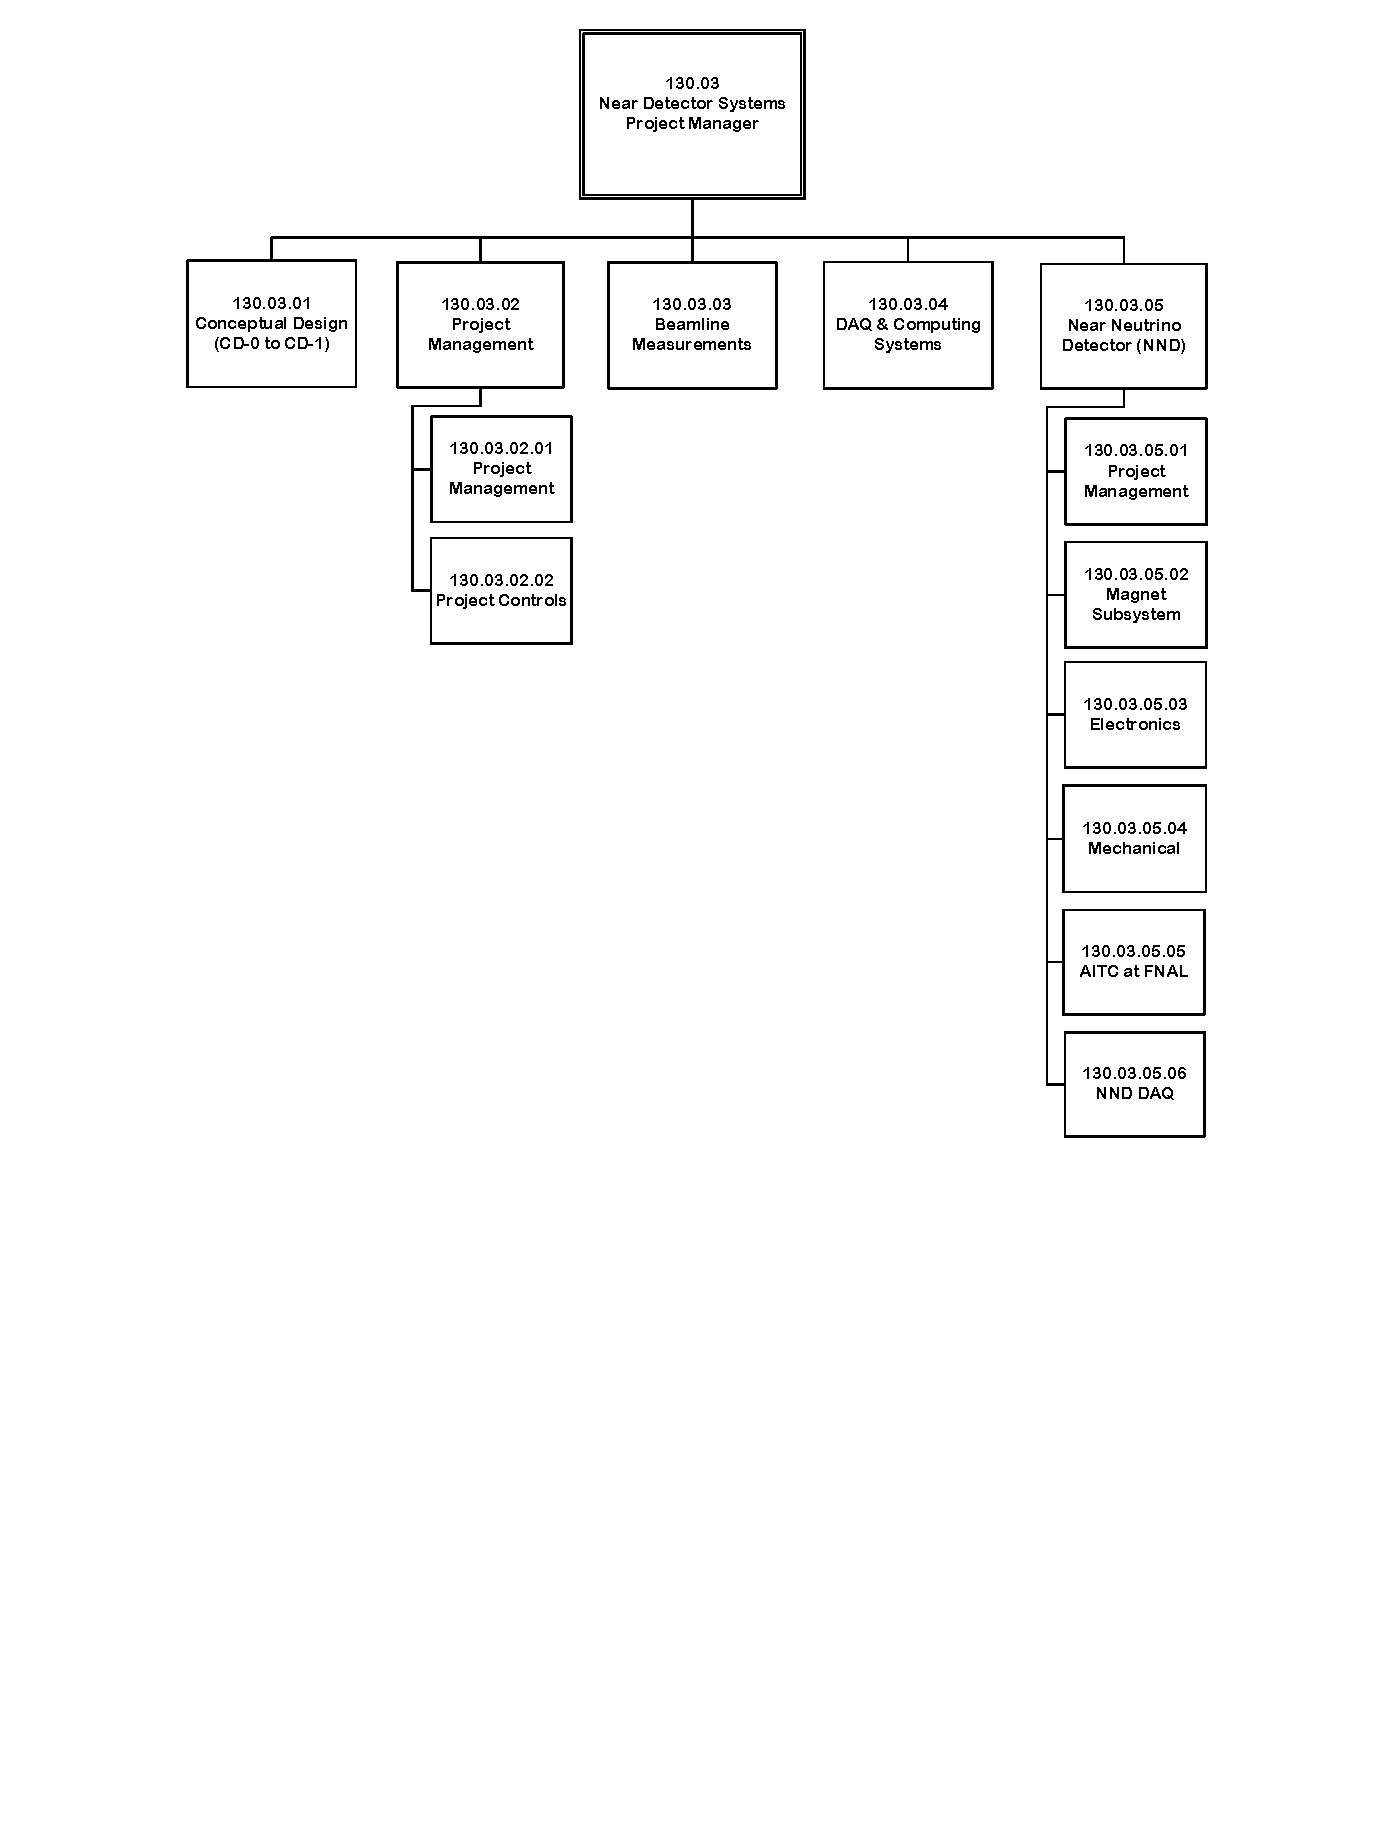
\includegraphics[width=0.85\textwidth]{ND_documents_nonames.pdf}
\end{center}
\end{cdrfigure}
\begin{cdrfigure}[Far detector WBS]{FD_WBS}{Far detector Work Breakdown Structure.}
\centering
\begin{center}
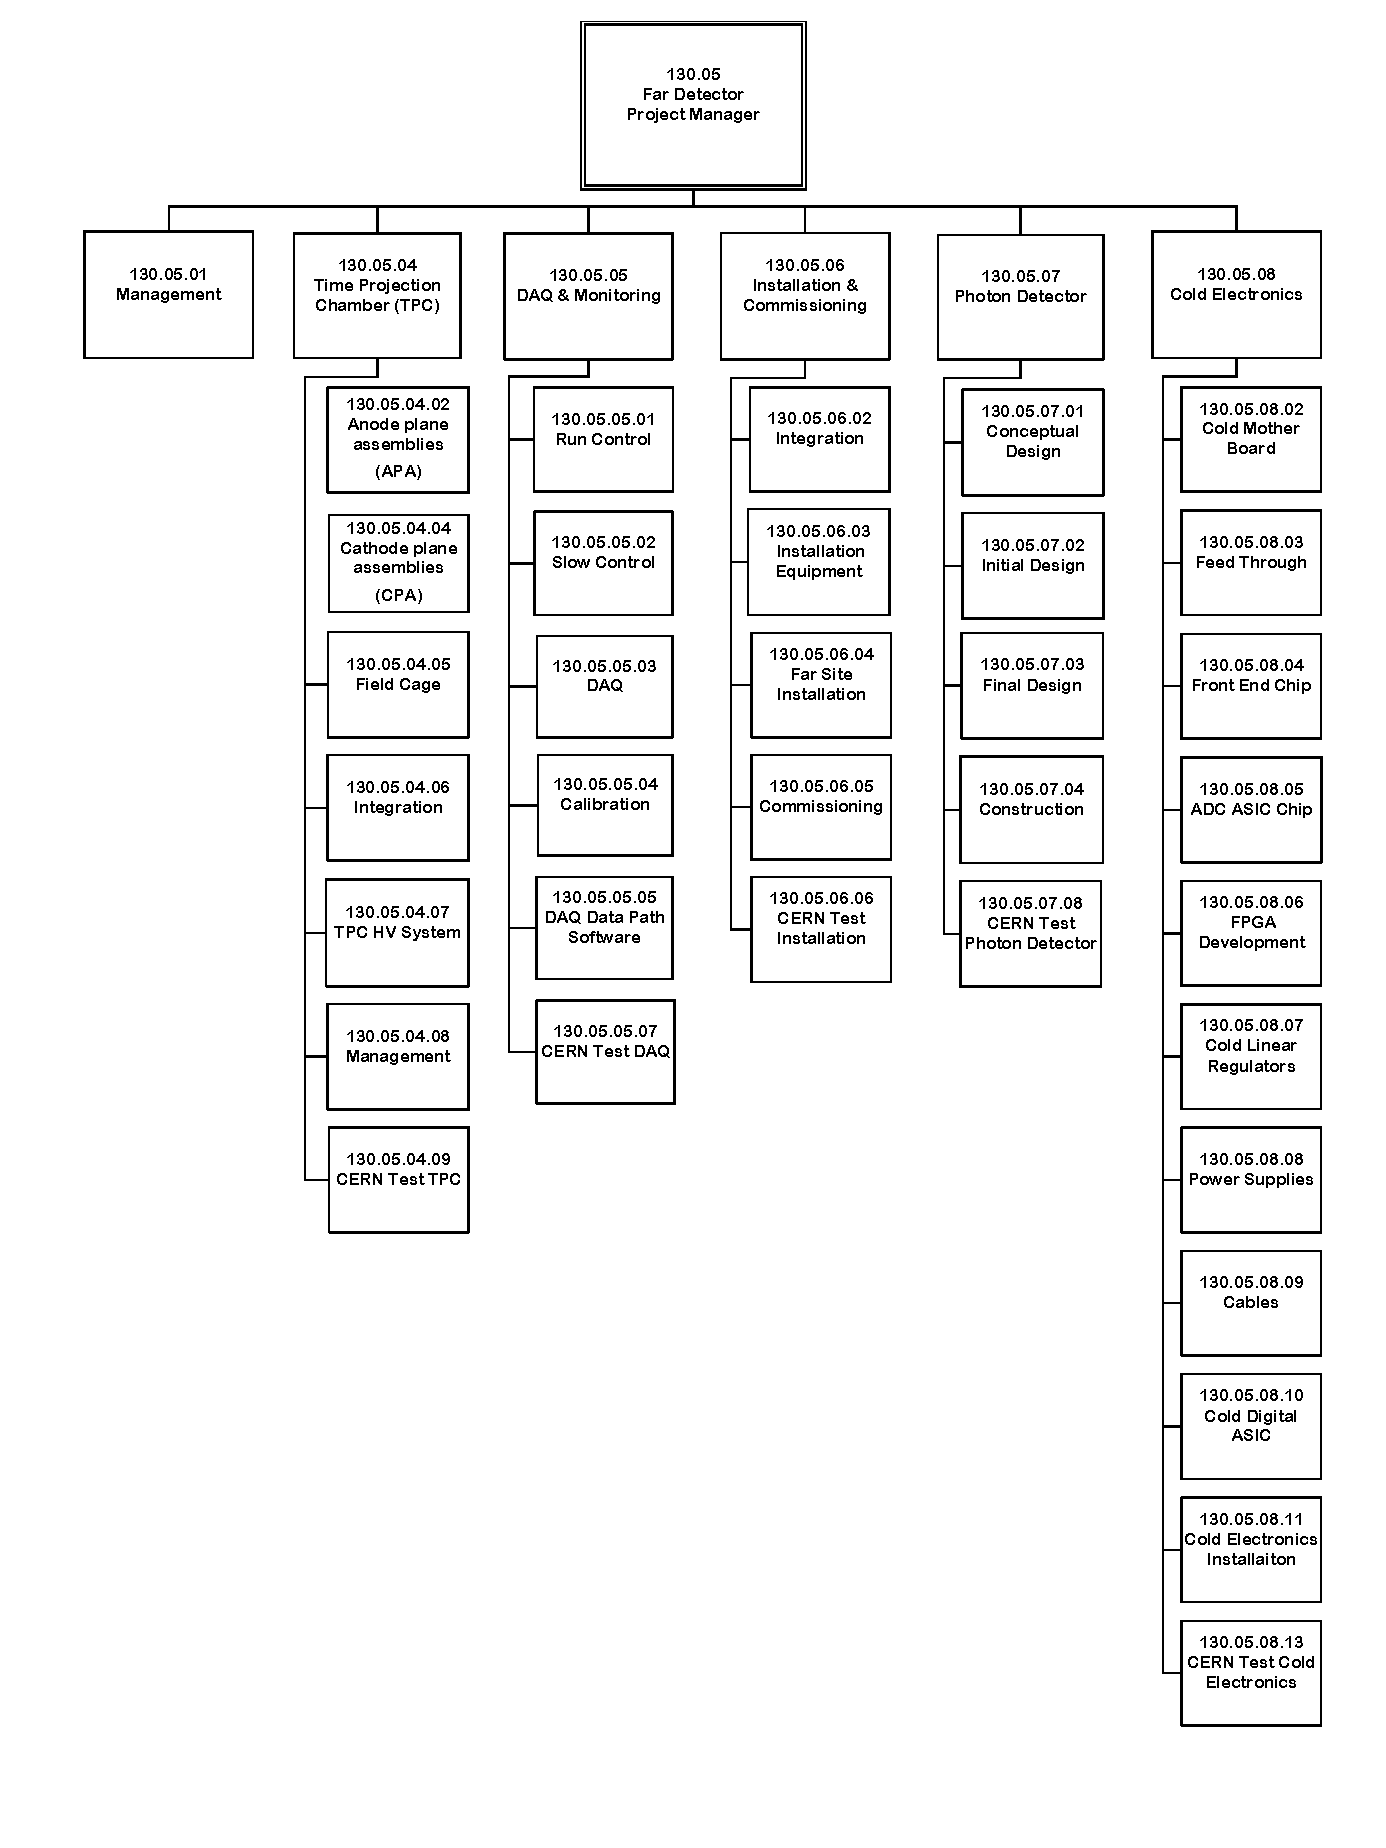
\includegraphics[width=0.9\textwidth]{FD_documents_nonames.pdf}
\end{center}
\end{cdrfigure}
The DUNE Project organization and structure will evolve as the project
becomes more fully internationalized.
